
\documentclass[11pt]{article}
\usepackage[hmargin=1in,vmargin=1in]{geometry}
\usepackage{xcolor}
\usepackage{mdframed}
\newmdenv[linecolor=blue,backgroundcolor=blue!10]{mybox}
\usepackage{tikz}
\usepackage{adjustbox}

\usetikzlibrary{shapes,arrows}
\usepackage{enumitem}
\usepackage{amsmath,amssymb,amsfonts,url,sectsty,framed,tcolorbox,framed}
\newcommand{\pf}{{\bf Proof: }}
\newtheorem{theorem}{Theorem}
\newtheorem{lemma}{Lemma}
\newtheorem{proposition}{Proposition}
\newtheorem{definition}{Definition}
\newtheorem{remark}{Remark}
\newcommand{\qed}{\hfill \rule{2mm}{2mm}}
\usepackage{enumitem}



\begin{document}
%%%%%%%%%%%%%%%%%%%%%%%%%%%%%%%%%%%%%%%%%%%%%%%%%%%%%%%%%%%%%%%%%%%%%
\noindent
\rule{\textwidth}{1pt}
\begin{center}
{\bf [CS304] Introduction to Cryptography and Network Security}
\end{center}
Course Instructor: Dr. Dibyendu Roy \hfill Winter 2023-2024\\
Scribed by: Manas Jitendrakumar Ingle (202151086) \hfill Lecture 1,2 (Week 5)
\\
\rule{\textwidth}{1pt}
%%%%%%%%%%%%%%%%%%%%%%%%%%%%%%%%%%%%%%%%%%%%%%%%%%%%%%%%%%%
%write here

\section{Advanced Encryption Standard:}
\begin{itemize}
    \item It is Standardized by NIST.
    \item Rijndael - winner of Advanced Encryption Standard Competition.
    \item Winner of the Competition was named AES.
\end{itemize}
AES is based on -
\begin{enumerate}
    \item Iterative block cipher.
    \item It is based on SPN.
\end{enumerate}
\subsection*{Types of AES:}
\begin{enumerate}
    \item \textbf{AES - 128}
    \begin{enumerate}
        \item Block size = 128 bit
        \item Number of Rounds = 10
        \item Secret key size = 128 bit
    \end{enumerate}
    \item \textbf{AES - 192}
    \begin{enumerate}
        \item Block size = 128 bit
        \item Number of Rounds = 12
        \item Secret key size = 192 bit
    \end{enumerate}
    \item \textbf{AES - 256}
    \begin{enumerate}
        \item Block size = 128 bit
        \item Number of Rounds = 14
        \item Secret key size = 256 bit
    \end{enumerate}
\end{enumerate}



\section{AES 128}

\begin{center}
    \tikzset{every picture/.style={line width=0.75pt}}
    
    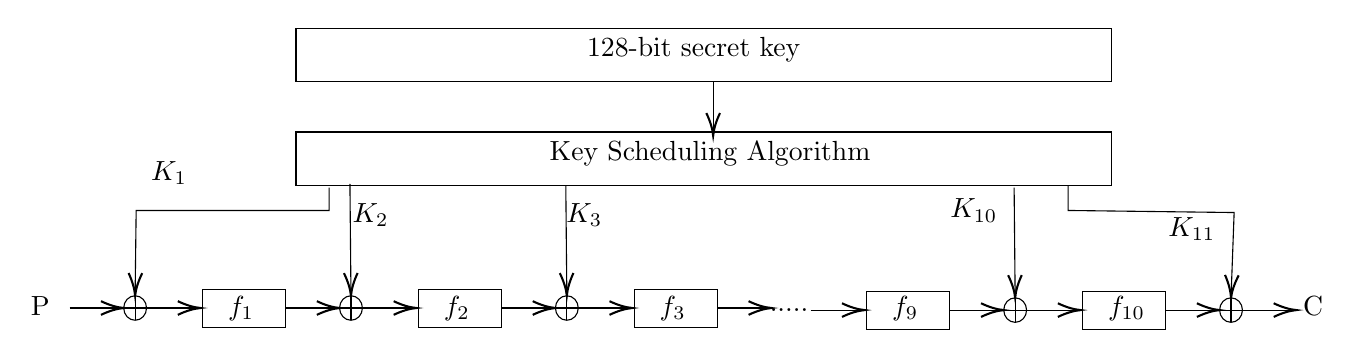
\begin{tikzpicture}[x=0.75pt,y=0.75pt,yscale=-1,xscale=1]
        \draw   (146,38) -- (539,38) -- (539,63.8) -- (146,63.8) -- cycle ;
        \draw    (347,63.8) -- (347,87.8) ;
        \draw [shift={(347,89.8)}, rotate = 270] [color={rgb, 255:red, 0; green, 0; blue, 0 }  ][line width=0.75]    (10.93,-3.29) .. controls (6.95,-1.4) and (3.31,-0.3) .. (0,0) .. controls (3.31,0.3) and (6.95,1.4) .. (10.93,3.29)   ; 
        \draw   (146,88) -- (539,88) -- (539,113.8) -- (146,113.8) -- cycle ;
        \draw    (37,172.8) -- (61,172.8) ;
        \draw [shift={(63,172.8)}, rotate = 180] [color={rgb, 255:red, 0; green, 0; blue, 0 }  ][line width=0.75]    (10.93,-3.29) .. controls (6.95,-1.4) and (3.31,-0.3) .. (0,0) .. controls (3.31,0.3) and (6.95,1.4) .. (10.93,3.29)   ;
        \draw   (63,172.8) .. controls (63,169.54) and (65.46,166.9) .. (68.5,166.9) .. controls (71.54,166.9) and (74,169.54) .. (74,172.8) .. controls (74,176.06) and (71.54,178.7) .. (68.5,178.7) .. controls (65.46,178.7) and (63,176.06) .. (63,172.8) -- cycle ; \draw   (63,172.8) -- (74,172.8) ; \draw   (68.5,166.9) -- (68.5,178.7) ;
        \draw    (74,172.8) -- (98,172.8) ;
        \draw [shift={(100,172.8)}, rotate = 180] [color={rgb, 255:red, 0; green, 0; blue, 0 }  ][line width=0.75]    (10.93,-3.29) .. controls (6.95,-1.4) and (3.31,-0.3) .. (0,0) .. controls (3.31,0.3) and (6.95,1.4) .. (10.93,3.29)   ;
        \draw   (101,163.8) -- (141,163.8) -- (141,182) -- (101,182) -- cycle ;
        \draw    (141,172.8) -- (165,172.8) ;
        \draw [shift={(167,172.8)}, rotate = 180] [color={rgb, 255:red, 0; green, 0; blue, 0 }  ][line width=0.75]    (10.93,-3.29) .. controls (6.95,-1.4) and (3.31,-0.3) .. (0,0) .. controls (3.31,0.3) and (6.95,1.4) .. (10.93,3.29)   ;
        \draw   (167,172.8) .. controls (167,169.54) and (169.46,166.9) .. (172.5,166.9) .. controls (175.54,166.9) and (178,169.54) .. (178,172.8) .. controls (178,176.06) and (175.54,178.7) .. (172.5,178.7) .. controls (169.46,178.7) and (167,176.06) .. (167,172.8) -- cycle ; \draw   (167,172.8) -- (178,172.8) ; \draw   (172.5,166.9) -- (172.5,178.7) ;
        \draw    (178,172.8) -- (202,172.8) ;
        \draw [shift={(204,172.8)}, rotate = 180] [color={rgb, 255:red, 0; green, 0; blue, 0 }  ][line width=0.75]    (10.93,-3.29) .. controls (6.95,-1.4) and (3.31,-0.3) .. (0,0) .. controls (3.31,0.3) and (6.95,1.4) .. (10.93,3.29)   ; 
        \draw   (205,163.8) -- (245,163.8) -- (245,182) -- (205,182) -- cycle ; 
        \draw    (245,172.8) -- (269,172.8) ;
        \draw [shift={(271,172.8)}, rotate = 180] [color={rgb, 255:red, 0; green, 0; blue, 0 }  ][line width=0.75]    (10.93,-3.29) .. controls (6.95,-1.4) and (3.31,-0.3) .. (0,0) .. controls (3.31,0.3) and (6.95,1.4) .. (10.93,3.29)   ; 
        \draw   (271,172.8) .. controls (271,169.54) and (273.46,166.9) .. (276.5,166.9) .. controls (279.54,166.9) and (282,169.54) .. (282,172.8) .. controls (282,176.06) and (279.54,178.7) .. (276.5,178.7) .. controls (273.46,178.7) and (271,176.06) .. (271,172.8) -- cycle ; \draw   (271,172.8) -- (282,172.8) ; \draw   (276.5,166.9) -- (276.5,178.7) ;
        \draw    (282,172.8) -- (306,172.8) ;
        \draw [shift={(308,172.8)}, rotate = 180] [color={rgb, 255:red, 0; green, 0; blue, 0 }  ][line width=0.75]    (10.93,-3.29) .. controls (6.95,-1.4) and (3.31,-0.3) .. (0,0) .. controls (3.31,0.3) and (6.95,1.4) .. (10.93,3.29)   ;
        \draw   (309,163.8) -- (349,163.8) -- (349,182) -- (309,182) -- cycle ;
        \draw    (349,172.8) -- (373,172.8) ;
        \draw [shift={(375,172.8)}, rotate = 180] [color={rgb, 255:red, 0; green, 0; blue, 0 }  ][line width=0.75]    (10.93,-3.29) .. controls (6.95,-1.4) and (3.31,-0.3) .. (0,0) .. controls (3.31,0.3) and (6.95,1.4) .. (10.93,3.29)   ;
        \draw    (394,173.8) -- (418,173.8) ;
        \draw [shift={(420,173.8)}, rotate = 180] [color={rgb, 255:red, 0; green, 0; blue, 0 }  ][line width=0.75]    (10.93,-3.29) .. controls (6.95,-1.4) and (3.31,-0.3) .. (0,0) .. controls (3.31,0.3) and (6.95,1.4) .. (10.93,3.29)   ;
        \draw   (421,164.8) -- (461,164.8) -- (461,183) -- (421,183) -- cycle ;
        \draw    (461,173.8) -- (485,173.8) ;
        \draw [shift={(487,173.8)}, rotate = 180] [color={rgb, 255:red, 0; green, 0; blue, 0 }  ][line width=0.75]    (10.93,-3.29) .. controls (6.95,-1.4) and (3.31,-0.3) .. (0,0) .. controls (3.31,0.3) and (6.95,1.4) .. (10.93,3.29)   ;
        \draw   (487,173.8) .. controls (487,170.54) and (489.46,167.9) .. (492.5,167.9) .. controls (495.54,167.9) and (498,170.54) .. (498,173.8) .. controls (498,177.06) and (495.54,179.7) .. (492.5,179.7) .. controls (489.46,179.7) and (487,177.06) .. (487,173.8) -- cycle ; \draw   (487,173.8) -- (498,173.8) ; \draw   (492.5,167.9) -- (492.5,179.7) ;
        \draw    (498,173.8) -- (522,173.8) ;
        \draw [shift={(524,173.8)}, rotate = 180] [color={rgb, 255:red, 0; green, 0; blue, 0 }  ][line width=0.75]    (10.93,-3.29) .. controls (6.95,-1.4) and (3.31,-0.3) .. (0,0) .. controls (3.31,0.3) and (6.95,1.4) .. (10.93,3.29)   ;
        \draw   (525,164.8) -- (565,164.8) -- (565,183) -- (525,183) -- cycle ;
        \draw    (565,173.8) -- (589,173.8) ;
        \draw [shift={(591,173.8)}, rotate = 180] [color={rgb, 255:red, 0; green, 0; blue, 0 }  ][line width=0.75]    (10.93,-3.29) .. controls (6.95,-1.4) and (3.31,-0.3) .. (0,0) .. controls (3.31,0.3) and (6.95,1.4) .. (10.93,3.29)   ;
        \draw   (591,173.8) .. controls (591,170.54) and (593.46,167.9) .. (596.5,167.9) .. controls (599.54,167.9) and (602,170.54) .. (602,173.8) .. controls (602,177.06) and (599.54,179.7) .. (596.5,179.7) .. controls (593.46,179.7) and (591,177.06) .. (591,173.8) -- cycle ; \draw   (591,173.8) -- (602,173.8) ; \draw   (596.5,167.9) -- (596.5,179.7) ; 
        \draw    (602,173.8) -- (626,173.8) ;
        \draw [shift={(628,173.8)}, rotate = 180] [color={rgb, 255:red, 0; green, 0; blue, 0 }  ][line width=0.75]    (10.93,-3.29) .. controls (6.95,-1.4) and (3.31,-0.3) .. (0,0) .. controls (3.31,0.3) and (6.95,1.4) .. (10.93,3.29)   ;
        \draw    (162,114.8) -- (162,125.8) -- (69,125.8) -- (68.52,164.9) ;
        \draw [shift={(68.5,166.9)}, rotate = 270.7] [color={rgb, 255:red, 0; green, 0; blue, 0 }  ][line width=0.75]    (10.93,-3.29) .. controls (6.95,-1.4) and (3.31,-0.3) .. (0,0) .. controls (3.31,0.3) and (6.95,1.4) .. (10.93,3.29)   ;
        \draw    (172,113) -- (172.48,164.9) ;
        \draw [shift={(172.5,166.9)}, rotate = 269.47] [color={rgb, 255:red, 0; green, 0; blue, 0 }  ][line width=0.75]    (10.93,-3.29) .. controls (6.95,-1.4) and (3.31,-0.3) .. (0,0) .. controls (3.31,0.3) and (6.95,1.4) .. (10.93,3.29)   ;
        \draw    (276,113.8) -- (276.48,164.9) ;
        \draw [shift={(276.5,166.9)}, rotate = 269.46] [color={rgb, 255:red, 0; green, 0; blue, 0 }  ][line width=0.75]    (10.93,-3.29) .. controls (6.95,-1.4) and (3.31,-0.3) .. (0,0) .. controls (3.31,0.3) and (6.95,1.4) .. (10.93,3.29)   ;
        \draw    (492,114.8) -- (492.48,165.9) ;
        \draw [shift={(492.5,167.9)}, rotate = 269.46] [color={rgb, 255:red, 0; green, 0; blue, 0 }  ][line width=0.75]    (10.93,-3.29) .. controls (6.95,-1.4) and (3.31,-0.3) .. (0,0) .. controls (3.31,0.3) and (6.95,1.4) .. (10.93,3.29)   ;
        \draw    (518,113.8) -- (518,125.8) -- (598,126.8) -- (596.57,165.9) ;
        \draw [shift={(596.5,167.9)}, rotate = 272.09] [color={rgb, 255:red, 0; green, 0; blue, 0 }  ][line width=0.75]    (10.93,-3.29) .. controls (6.95,-1.4) and (3.31,-0.3) .. (0,0) .. controls (3.31,0.3) and (6.95,1.4) .. (10.93,3.29)   ;
        
        \draw (285,41) node [anchor=north west][inner sep=0.75pt]   [align=left] {128-bit secret key};
        \draw (267,91) node [anchor=north west][inner sep=0.75pt]   [align=left] {Key Scheduling Algorithm};
        \draw (17,166) node [anchor=north west][inner sep=0.75pt]   [align=left] {P};
        \draw (112,166) node [anchor=north west][inner sep=0.75pt]   [align=left] {$f_1$};
        \draw (216,166) node [anchor=north west][inner sep=0.75pt]   [align=left] {$f_2$};
        \draw (320,166) node [anchor=north west][inner sep=0.75pt]   [align=left] {$f_3$};
        \draw (373,172) node [anchor=north west][inner sep=0.75pt]   [align=left] {.....};
        \draw (432,166) node [anchor=north west][inner sep=0.75pt]   [align=left] {$f_9$};
        \draw (536,166) node [anchor=north west][inner sep=0.75pt]   [align=left] {$f_{10}$};
        \draw (630,166) node [anchor=north west][inner sep=0.75pt]   [align=left] {C};
        \draw (75,101) node [anchor=north west][inner sep=0.75pt]   [align=left] {$K_1$};
        \draw (172,121) node [anchor=north west][inner sep=0.75pt]   [align=left] {$K_2$};
        \draw (275,121) node [anchor=north west][inner sep=0.75pt]   [align=left] {$K_3$};
        \draw (460,119) node [anchor=north west][inner sep=0.75pt]   [align=left] {$K_{10}$};
        \draw (565,128) node [anchor=north west][inner sep=0.75pt]   [align=left] {$K_{11}$};
    \end{tikzpicture}
\end{center}

The diagram illustrates the process of encrypting plaintext using the AES 128 algorithm. The encryption begins with a 128-bit secret key, which undergoes a Key Scheduling Algorithm to generate 11 round keys, each also 128 bits in length. 

The plaintext, denoted as P, is then XOR-ed with the first round key, denoted as $K_1$. This intermediate result is fed into the first round function, $f_1$, which produces a 128-bit output. This output is further processed by XOR-ing with the second round key, $K_2$, and then passed through the second round function, $f_2$. This process iterates through $f_3$ to $f_{10}$, with each function generating a new output and XOR-ing it with the corresponding round key.

Finally, the output of the tenth round function, $f_{10}$, undergoes XOR with the eleventh round key, $K_{11}$, to produce the ciphertext, denoted as C.

\vspace{3mm}
Given the ciphertext, decryption process will begin with xoring the ciphertext with $K_{11}$(last round key) and this output will be input to inverse of $f_{10}$ function. Inverse of $f_{10}$ function will generate a 128-bit output which will be xored with $K_{10}$, and output will be passed to inverse of $f_9$ function, and so on it will be continued till inverse of $f_1$ function. The output will be xored with $K_1$(first round key) to get the plaintext.\\
\newline
\textbf{Note:} The decryption process described above clearly states that the round functions $f_1, f_2,..., f_{10}$ must be invertible. Hence, this structure is different from Feistel Network where the invertibility of round functions does not matter. \\
Now, we need to understand the following things:
\begin{itemize}
    \item Round Functions
    \item Key Scheduling Algorithm
\end{itemize}


        \subsection*{Round Functions of AES-128:}  
        $f_1, f_2,\dots, f_{10}$ 
        \begin{enumerate}
            \item $f_1 = f_2 = f_3 \dots = f_9$ 
            \item $f_{10}$ is different from $f_i, i = 1,2,\dots, 9$ \\
        \end{enumerate}
         First 9 round functions are exactly same and the $10^{th}$ round function is different from other 9 round functions.
         \begin{itemize}
         \item The first 9 round functions $(i.e, f_1, f_2, \dots, f_9)$ are based on the following functions:
         \begin{enumerate}
             \item Sub-bytes \hfill $f_i: \{\ 0,1 \}\ ^{128} \to \{\ 0,1 \}\ ^{128} $
             \item Shift rows \hfill $Mix col(Shift rows(sub-bytes(x))) = f_i(x)$
             \item Mix columns
         \end{enumerate}
         The $10^{th}$ round function $(i.e, f_{10})$ is based on: 
         \begin{enumerate}
             \item Sub-bytes \hfill $f_{10}: \{\ 0,1 \}\ ^{128} \to \{\ 0,1 \}\ ^{128} $
             \item Shift rows
         \end{enumerate}
         The only difference between the last round function and the rest is that the last round function do not make use of mix columns.
          \end{itemize}

\begin{adjustbox}{max totalsize={.9\textwidth}{.8\textheight},center}
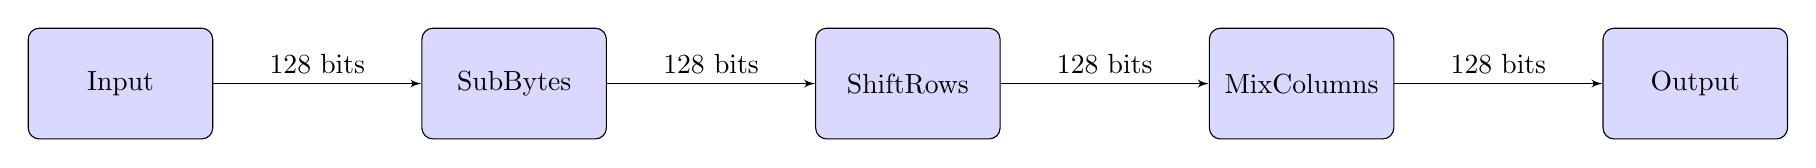
\begin{tikzpicture}[auto, node distance=5cm,>=latex']
    \tikzstyle{block} = [rectangle, draw, fill=blue!15, 
        text width=6em, text centered, rounded corners, minimum height=4em]
    \tikzstyle{line} = [draw, -latex']

    \node [block] (input) {Input};
    \node [block, right of=input] (subbytes) {SubBytes};
    \node [block, right of=subbytes] (shiftrows) {ShiftRows};
    \node [block, right of=shiftrows] (mixcolumns) {MixColumns};
    \node [block, right of=mixcolumns] (output) {Output};

    \path [line] (input) -- node[midway,above] {128 bits} (subbytes);
    \path [line] (subbytes) -- node[midway,above] {128 bits} (shiftrows);
    \path [line] (shiftrows) -- node[midway,above] {128 bits} (mixcolumns);
    \path [line] (mixcolumns) -- node[midway,above] {128 bits} (output);
\end{tikzpicture}
\end{adjustbox}

\begin{center}
    \tikzset{every picture/.style={line width=0.75pt}} 
    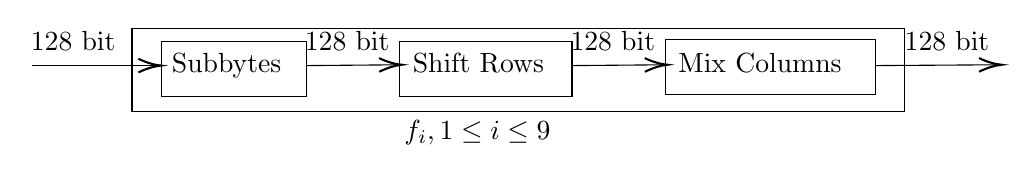
\begin{tikzpicture}[x=0.75pt,y=0.75pt,yscale=-1,xscale=1]
        \draw   (139,298.6) -- (511,298.6) -- (511,338.6) -- (139,338.6) -- cycle ;
        \draw   (153,305.2) -- (223,305.2) -- (223,331.6) -- (153,331.6) -- cycle ;
        \draw   (268,305.2) -- (351,305.2) -- (351,331.6) -- (268,331.6) -- cycle ;
        \draw   (396,304.2) -- (497,304.2) -- (497,330.6) -- (396,330.6) -- cycle ;
        \draw    (223,316.6) -- (267,316.22) ;
        \draw [shift={(269,316.2)}, rotate = 179.5] [color={rgb, 255:red, 0; green, 0; blue, 0 }  ][line width=0.75]    (10.93,-3.29) .. controls (6.95,-1.4) and (3.31,-0.3) .. (0,0) .. controls (3.31,0.3) and (6.95,1.4) .. (10.93,3.29)   ;
        \draw    (351,316.6) -- (395,316.22) ;
        \draw [shift={(397,316.2)}, rotate = 179.5] [color={rgb, 255:red, 0; green, 0; blue, 0 }  ][line width=0.75]    (10.93,-3.29) .. controls (6.95,-1.4) and (3.31,-0.3) .. (0,0) .. controls (3.31,0.3) and (6.95,1.4) .. (10.93,3.29)   ;
        \draw    (91,316.6) -- (151,316.6) ;
        \draw [shift={(153,316.6)}, rotate = 180] [color={rgb, 255:red, 0; green, 0; blue, 0 }  ][line width=0.75]    (10.93,-3.29) .. controls (6.95,-1.4) and (3.31,-0.3) .. (0,0) .. controls (3.31,0.3) and (6.95,1.4) .. (10.93,3.29)   ;
        \draw    (497,316.6) -- (556,316.21) ;
        \draw [shift={(558,316.2)}, rotate = 179.62] [color={rgb, 255:red, 0; green, 0; blue, 0 }  ][line width=0.75]    (10.93,-3.29) .. controls (6.95,-1.4) and (3.31,-0.3) .. (0,0) .. controls (3.31,0.3) and (6.95,1.4) .. (10.93,3.29)   ;
        
        \draw (157,309.2) node [anchor=north west][inner sep=0.75pt]   [align=left] {Subbytes};
        \draw (273,309.2) node [anchor=north west][inner sep=0.75pt]   [align=left] {Shift Rows};
        \draw (401,309.2) node [anchor=north west][inner sep=0.75pt]   [align=left] {Mix Columns};
        \draw (221,298.6) node [anchor=north west][inner sep=0.75pt]   [align=left] {128 bit};
        \draw (349,298.6) node [anchor=north west][inner sep=0.75pt]   [align=left] {128 bit};
        \draw (89,298.6) node [anchor=north west][inner sep=0.75pt]   [align=left] {128 bit};
        \draw (510,298.6) node [anchor=north west][inner sep=0.75pt]   [align=left] {128 bit};
        \draw (269,341.6) node [anchor=north west][inner sep=0.75pt]   [align=left] {$f_i, 1 \leq i \leq 9$};
    \end{tikzpicture}
\end{center}

\begin{center}
    \caption{Block Diagram for AES-128 for first 9 rounds}
\end{center}


    
\begin{adjustbox}{max totalsize={.9\textwidth}{.8\textheight},center}
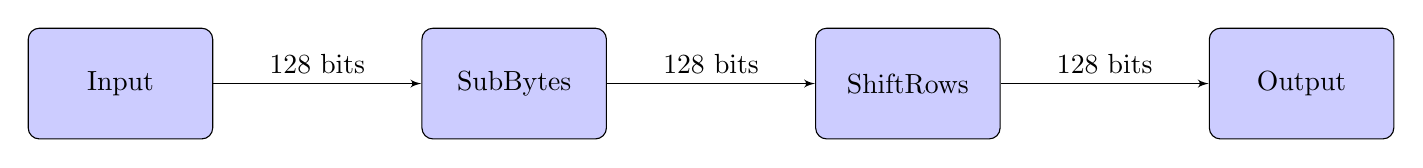
\begin{tikzpicture}[auto, node distance=5cm,>=latex']
    \tikzstyle{block} = [rectangle, draw, fill=blue!20, 
        text width=6em, text centered, rounded corners, minimum height=4em]
    \tikzstyle{line} = [draw, -latex']

    \node [block] (input) {Input};
    \node [block, right of=input] (subbytes) {SubBytes};
    \node [block, right of=subbytes] (shiftrows) {ShiftRows};
    
    \node [block, right of=shiftrows] (output) {Output};

    \path [line] (input) -- node[midway,above] {128 bits} (subbytes);
    \path [line] (subbytes) -- node[midway,above] {128 bits} (shiftrows);
    \path [line] (shiftrows) -- node[midway,above] {128 bits} (output);
\end{tikzpicture}
\end{adjustbox}

\begin{center}
    \tikzset{every picture/.style={line width=0.75pt}} 

    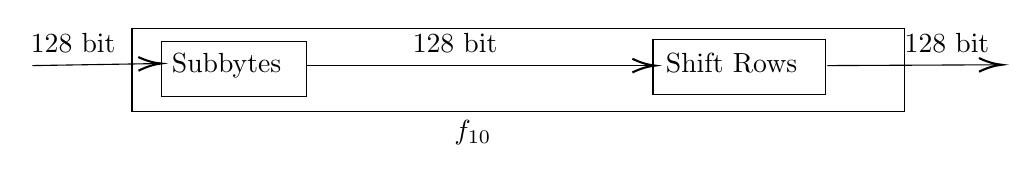
\begin{tikzpicture}[x=0.75pt,y=0.75pt,yscale=-1,xscale=1] 
        \draw   (146,426.6) -- (518,426.6) -- (518,466.6) -- (146,466.6) -- cycle ;
        \draw   (160,433.2) -- (230,433.2) -- (230,459.6) -- (160,459.6) -- cycle ;
        \draw   (397,432.2) -- (480,432.2) -- (480,458.6) -- (397,458.6) -- cycle ;
        \draw    (230,444.6) -- (396,444.6) ;
        \draw [shift={(398,444.6)}, rotate = 180] [color={rgb, 255:red, 0; green, 0; blue, 0 }  ][line width=0.75]    (10.93,-3.29) .. controls (6.95,-1.4) and (3.31,-0.3) .. (0,0) .. controls (3.31,0.3) and (6.95,1.4) .. (10.93,3.29)   ; 
        \draw    (98,444.6) -- (158,443.63) ;
        \draw [shift={(160,443.6)}, rotate = 179.08] [color={rgb, 255:red, 0; green, 0; blue, 0 }  ][line width=0.75]    (10.93,-3.29) .. controls (6.95,-1.4) and (3.31,-0.3) .. (0,0) .. controls (3.31,0.3) and (6.95,1.4) .. (10.93,3.29)   ;
        \draw    (481,444.6) -- (563,444.21) ;
        \draw [shift={(565,444.2)}, rotate = 179.73] [color={rgb, 255:red, 0; green, 0; blue, 0 }  ][line width=0.75]    (10.93,-3.29) .. controls (6.95,-1.4) and (3.31,-0.3) .. (0,0) .. controls (3.31,0.3) and (6.95,1.4) .. (10.93,3.29)   ;
        
        \draw (164,437.2) node [anchor=north west][inner sep=0.75pt]   [align=left] {Subbytes};
        \draw (402,437.2) node [anchor=north west][inner sep=0.75pt]   [align=left] {Shift Rows};
        \draw (280,427.6) node [anchor=north west][inner sep=0.75pt]   [align=left] {128 bit};
        \draw (96,427.6) node [anchor=north west][inner sep=0.75pt]   [align=left] {128 bit};
        \draw (517,427.6) node [anchor=north west][inner sep=0.75pt]   [align=left] {128 bit};
        \draw (300,469.6) node [anchor=north west][inner sep=0.75pt]   [align=left] {$f_{10}$};
    \end{tikzpicture}
\end{center}

\begin{center}
    \caption{For the Last Round function $f_{10}$}
\end{center}

\subsection*{Subbytes}
Subbytes is a bijective mapping from 128-bit to 128-bit.

Let $X = x_0 x_1 \ldots x_{15}$ where the size of each $x_i$ is 8 bits. 


\text{X} \xrightarrow{Mapping} \text{S} 
\newline
\begin{bmatrix}
x_0 & x_1 & x_2 & x_3 \\
x_4 & x_5 & x_6 & x_7 \\
x_8 & x_9 & x_{10} & x_{11} \\
x_{12} & x_{13} & x_{14} & x_{15}
\end{bmatrix} 
\xrightarrow{}
\begin{bmatrix}
S_{00} & S_{01} & S_{02} & S_{03} \\
S_{10} & S_{11} & S_{12} & S_{13} \\
S_{20} & S_{21} & S_{22} & S_{23} \\
S_{30} & S_{31} & S_{32} & S_{33}
\end{bmatrix} 

\textbf{S-Box Definition:}

$S : \{0, 1\}^8 \rightarrow \{0, 1\}^8$

\textbf{S-Box Initialization:}

$S(0) = 0$

\textbf{Hexadecimal Representation of Constants:}

C = $C_7C_6C_5C_4C_3C_2C_1C_0 $ \leftarrow $(01100011) = (63)_{16}$

\textbf{S-Box Transformation:}

For an input $s_{ij}$ represented as $(a_7a_6a_5a_4a_3a_2a_1a_0)$:

\[ b_i = (a_i + a_{i+4} \mod 8 + a_{i+5} \mod 8 + a_{i+6} \mod 8 + a_{i+7} \mod 8 + C_i) \mod 2 \]

Output:

\[ s'_{ij} = (b_7b_6b_5b_4b_3b_2b_1b_0) \]

Hence, $S'_{ij}$ is computed for each $S_{ij}$ and the output matrix is the output of subbyte function.
\begin{center}
    $
    \begin{bmatrix}
        S_{00} & S_{01} & S_{02} & S_{03}\\
        S_{10} & S_{11} & S_{12} & S_{13}\\
        S_{20} & S_{21} & S_{22} & S_{23}\\
        S_{30} & S_{31} & S_{32} & S_{33}\\
    \end{bmatrix}
    \xrightarrow{Subbyte}
    \begin{bmatrix}
        S'_{00} & S'_{01} & S'_{02} & S'_{03}\\
        S'_{10} & S'_{11} & S'_{12} & S'_{13}\\
        S'_{20} & S'_{21} & S'_{22} & S'_{23}\\
        S'_{30} & S'_{31} & S'_{32} & S'_{33}\\
    \end{bmatrix}
    $
\end{center}

\subsubsection{Mix Columns}
Mix columns, again, is a mapping from 128-bit to 128-bit. It also takes a $4 \times 4$ matrix as input (the output of Shift Rows function).
\begin{center}
    Mix Columns: $\{0, 1\}^{128} \rightarrow \{0, 1\}^{128}$\\
    \vspace{1mm}
    $(S_{ij})_{4 \times 4} \xrightarrow{Mix Columns} (S_{ij}^{'})_{4 \times 4}$
\end{center}
Consider the column $c \in {0,1,2,3}$ of matrix S.
\begin{center}
    column = $\begin{bmatrix}
        S_{0c}\\
        S_{1c}\\
        S_{2c}\\
        S_{3c}\\
    \end{bmatrix}$
\end{center}
The Mix Columns function is defined as follows. For i = 0 to i = 3, let $t_i$ be the polynomial constructed from $S_{ic}$. Define four polynomials as:
\begin{center}
    $u_0 = [(x * t_0) + (x + 1) * t_1 + t_2 + t_3]$ mod $(x^8 + x^4 + x^3 + x + 1)$\\
    \vspace{1mm}
    $u_1 = [t_0 + (x * t_1) + (x + 1) * t_2 + t_3]$ mod $(x^8 + x^4 + x^3 + x + 1)$\\
    \vspace{1mm}
    $u_2 = [t_0 + t_1 + (x * t_2) + (x + 1) * t_3]$ mod $(x^8 + x^4 + x^3 + x + 1)$\\
    \vspace{1mm}
    $u_3 = [(x + 1) * t_0 + t_1 + t_2 + (x * t_3)]$ mod $(x^8 + x^4 + x^3 + x + 1)$\\
\end{center}
Now, $S_{ij}^{'}$ is the binary 8-bits constructed using $u_i$. Therefore, 
\begin{center}
    $\begin{bmatrix}
        S_{0c}\\
        S_{1c}\\
        S_{2c}\\
        S_{3c}\\
    \end{bmatrix}
    \xrightarrow{Mix Columns}
    \begin{bmatrix}
        S_{0c}^{'}\\
        S_{1c}^{'}\\
        S_{2c}^{'}\\
        S_{3c}^{'}\\
    \end{bmatrix}$
\end{center}
Applying Mix Columns to each columns, will give us the entire $(S_{ij}^{'})_{4 \times 4}$ matrix. Therefore, Mix Column can be defined as a matrix multiplication as:
\begin{center}
    $
    (S_{ij}^{'})_{4 \times 4} = 
    \begin{bmatrix}
        x & x + 1 & 1 & 1\\
        1 & x & x+1 & 1\\
        1 & 1 & x & x+1\\
        x+1 & 1 & 1 & x\\
    \end{bmatrix}
    \times
    \begin{bmatrix}
        S_{00} & S_{01} & S_{02} & S_{03}\\
        S_{10} & S_{11} & S_{12} & S_{13}\\
        S_{20} & S_{21} & S_{22} & S_{23}\\
        S_{30} & S_{31} & S_{32} & S_{33}\\
    \end{bmatrix}
    $
    mod $(x^8 + x^4 + x^3 + x + 1)$
\end{center}
In terms of hexadecimal, the above multiplication can be represented as:
\begin{center}
    $
    (S_{ij}^{'})_{4 \times 4} = 
    \begin{bmatrix}
        2 & 3 & 1 & 1\\
        1 & 2 & 3 & 1\\
        1 & 1 & 2 & 3\\
        3 & 1 & 1 & 2\\
    \end{bmatrix}
    \times
    \begin{bmatrix}
        S_{00} & S_{01} & S_{02} & S_{03}\\
        S_{10} & S_{11} & S_{12} & S_{13}\\
        S_{20} & S_{21} & S_{22} & S_{23}\\
        S_{30} & S_{31} & S_{32} & S_{33}\\
    \end{bmatrix}
    $
    mod $(x^8 + x^4 + x^3 + x + 1)$
\end{center}

The polynomial $(x^8 + x^4 + x^3 + x + 1)$ is a primitive polynomial, hence, it is possible to construct the inverse of the Mix Columns function.\\
\newpage

\rule{\textwidth}{1pt}
\begin{center}
    \textbf{Lecture 2} [16/02/24]
\end{center}
\rule{\textwidth}{1pt}


Find $\begin{bmatrix}
        S_{00}^{'}\\
        S_{10}^{'}\\
        S_{20}^{'}\\
        S_{30}^{'}\\
    \end{bmatrix}$ after doing the Mix Column operation on $\begin{bmatrix}
        S_{0c}\\
        S_{1c}\\
        S_{2c}\\
        S_{3c}\\
    \end{bmatrix}$ where $S_{00} = 95, S_{10} = 65, S_{20} = fd, S_{30} = f3$.\\

\textbf{Solution:}
\begin{center}
    $S_{00} = 95 = 10010101 = x^7 + x^4 + x^2 + 1$\\
    $S_{10} = 65 = 01100101 = x^6 + x^5 + x^2 + 1$\\
    $S_{20} = fd = 11111101 = x^7 + x^6 + x^5 + x^4 + x^3 + x^2 + 1$\\
    $S_{30} = f3 = 11110011 = x^7 + x^6 + x^5 + x^4 + x + 1$\\
\end{center}
Now, let's calculate $S_{00}^{'}$.\\
\newline
$S_{00}^{'} = (x * S_{00} + (x+1) * S_{10} + S_{20} + S_{30})$ mod $(x^8 + x^4 + x^3 + x + 1)$\\
\newline
$S_{00}^{'} = ((x^8 + x^5 + x^3 + x) + (x^7 + x^5 + x^3 + x^2 + x + 1) + S_{20} + S_{30})$ mod $(x^8 + x^4 + x^3 + x + 1)$\\
\newline
$S_{00}^{'} = (x^8 + x^7 + x^3 + x + 1)$ mod $(x^8 + x^4 + x^3 + x + 1)$\\
\newline
$S_{00}^{'} = (x^7 + x^4) = 10010000 = (90)_{16}$\\
\newline
Similarly we can compute $S_{10}^{'}, S_{20}^{'}$ and $S_{30}^{'}$. Let's calculate each one of them.\\
\newline
    $S_{10}^{'} = (S_{00} + x * S_{10} + (x + 1) * S_{20} + S_{30})$ mod $(x^8 + x^4 + x^3 + x + 1)$\\
    \newline
    $S_{10}^{'} = (S_{00} + (x^7 + x^6 + x^3 + x) + (x^8 + x^2 + x + 1) + S_{30})$ mod $(x^8 + x^4 + x^3 + x + 1)$\\
    \newline
    $S_{10}^{'} = (x^8 + x^7 + x^5 + x^3 + x + 1)$ mod $(x^8 + x^4 + x^3 + x + 1)$\\
    \newline
    $S_{10}^{'} = (x^7 + x^5 + x^4) = 10110000 = (b0)_{16}$\\
\newline
Similarly, \\
\newline
    $S_{20}^{'} = (S_{00} + S_{10} + x * S_{20} + (x+1) * S_{30})$ mod $(x^8 + x^4 + x^3 + x + 1)$\\
    \newline
    $S_{20}^{'} = (S_{00} + S_{10} + (x^8 + x^7 + x^6 + x^5 + x^4 + x^3 + x) + (x^8 + x^4 + x^2 + 1))$ mod $(x^8 + x^4 + x^3 + x + 1)$\\
    \newline
    $S_{20}^{'} = (x^4 + x^3 + x^2 + x + 1)$ mod $(x^8 + x^4 + x^3 + x + 1)$\\
    \newline
    $S_{20}^{'} = (x^4 + x^3 + x^2 + x + 1) = 00011111 = (1f)_{16}$\\
    \newline
Similarly,\\
\newline
    $S_{30}^{'} = ((x+1) * S_{00} + S_{10} + S_{20} + x * S_{30})$ mod $(x^8 + x^4 + x^3 + x + 1)$\\
    \newline
    $S_{30}^{'} = ((x^8 + x^7 + x^5 + x^4 + x^3 + x^2 + x + 1) + S_{10} + S_{20} + (x^8 + x^7 + x^6 + x^5 + x^2 + x))$ mod $(x^8 + x^4 + x^3 + x + 1)$\\
    \newline
    $S_{30}^{'} = (x^7 + x^6 + 1)$ mod $(x^8 + x^4 + x^3 + x + 1)$\\
    \newline
    $S_{30}^{'} = (x^7 + x^6 + 1) = 11000001 = (c1)_{16}$\\
\newline
Therefore, we have,
\begin{center}
    $
    \begin{bmatrix}
        S_{00}^{'}\\
        S_{10}^{'}\\
        S_{20}^{'}\\
        S_{30}^{'}\\
    \end{bmatrix}
    =
    \begin{bmatrix}
        90\\
        b0\\
        1f\\
        c1\\
    \end{bmatrix}
    $
\end{center}.

\subsection*{Key Scheduling Algorithm of AES 128}
The key scheduling algorithm of AES-128 takes 128-bit key as input and generate 11 round keys of 128-bits each.
\begin{center}
    key = $(key[0], key[1],....., key[15])$ where each $key[i]$ is 1 byte long
\end{center}
We will generate 44 words (32-bit) - w[0], w[1],...., w[43]. We can see that (32 * 44)/128 = 11. Therefore, we can generate 11 round keys from these 44 words.\\

There are two functions involved in key scheduling algorithm. These are given below:
\begin{enumerate}
    \item ROTWORD($B_0B_1B_2B_3$): It takes a word as input and performs left circular shift of its bytes once (or left circular shift by 8 bits). Here, $B_0, B_1, B_2, B_3$ are bytes of the input word. The output of the ROTWORD function is:
    \begin{center}
        ROTWORD($B_0B_1B_2B_3$) = $B_1B_2B_3B_0$
    \end{center}

    \item SUBWORD($B_0B_1B_2B_3$): It takes a word as input and performs the Subbyte function (defined in round function of AES) of its bytes $B_0, B_1, B_2, B_3$. The output of SUBWORD function is:
    \begin{center}
        SUBWORD($B_0B_1B_2B_3$) = $B_0^{'} B_1^{'} B_2^{'} B_3^{'}$\\
        where $B_i^{'} = Subbytes(B_i)$ $\forall$ $i \in \{0,1,2,3\}$
    \end{center}
\end{enumerate}
Also, there are ten round constants (which are words, i.e, 32-bit) defined as:
\begin{center}
    $RCON[1] = 01000000$\\
    $RCON[2] = 02000000$\\
    $RCON[3] = 04000000$\\
    $RCON[4] = 08000000$\\
    $RCON[5] = 10000000$\\
    $RCON[6] = 20000000$\\
    $RCON[7] = 40000000$\\
    $RCON[8] = 80000000$\\
    $RCON[9] = 1b000000$\\
    $RCON[10] = 36000000$\\
\end{center}
Note that the values of constants written above are in hexadecimal. The 44 words are generated using the below algorithm.

For \( i = 0 \) to 3:
\[
w[i] = (Key[4i], Key[4i + 1], Key[4i + 2], Key[4i + 3])
\]

For \( i = 4 \) to 43:
\[
\text{temp} = w[i - 1]
\]
if \( i \equiv 0 \mod 4 \):
\[
\text{temp} = \text{SUBWORD}(\text{ROTWORD}(\text{temp})) \oplus \text{Rcon}[i/4]
\]
\[
w[i] = w[i - 4] \oplus \text{temp}
\]

Now, the round keys will be given as:
\begin{center}
    $K_1 = w[0] || w[1] || w[2] || w[3]$\\
    \vspace{1mm}
    $K_2 = w[4] || w[5] || w[6] || w[7]$\\
    \vspace{1mm}
    .\\
    .\\
    $K_{11} = w[40] || w[41] || w[42] || w[43]$\\
    \vspace{1mm}
\end{center}

\subsection*{Mode of Operation}
We know that we can encrypt 128 bit blocks using AES at once. Suppose we want to encrypt more data, let's say 256 bit data. We need some mechanism to encrypt this data. There are certain mode of operations which we will be discussing in encrypting more data than the block length. Few examples of mode of operation are mentioned below.
\begin{enumerate}
    \item Electronic CodeBook Mode (EBC)
    \item Cipher FeedBack Mode (CFB)
    \item Cipher Block Chaining Mode (CBC)
    \item Output FeedBack Mode (OFB)
\end{enumerate}
\newline


\subsubsection*{Electronic CodeBook Mode}
As discussed above, in this mode, the plaintext is divided into continous blocks of l-bit size and each block is encrypted separately. The corresponding ciphertexts are concatenated in the same order to get the final ciphertext.
\begin{center}
    $M = m_0 || m_1 || ..... || m_t$ (plaintext)\\
    $len(m_i) = l-bit$ (each $m_i$ is a block, for AES, l = 128)
\end{center} 
\textbf{Encryption:}
\begin{center}
    $C = C_0 || C_1 || ..... || C_t$\\
    $C_i = Enc(m_i, K)$ $\forall$ $i \in \{0,1,...,t\}$
\end{center}
\textbf{Decryption:}
\begin{center}
    $M = m_0 || m_1 || ..... || m_t$\\
    $m_i = Dec(C_i, K)$ $\forall$ $i \in \{0,1,...,t\}$
\end{center}
The advantages of using ECB mode is that multiple blocks can be encrypted in parallel. However, it will reveal information if few blocks are same, i.e., if $m_i = m_j$ then $C_i = C_j$.

\subsubsection*{Cipher Block Chaining Mode}
It is the most used mode of operation. It is used in applications like WhatsApp. There is a block of l-bit which is public. It is known as Initialization Vector (IV).\\
\newline
\textbf{Encryption:}
\begin{center}
    $M = m_1 || m_2 || ..... || m_t$ (plaintext)\\
    $len(m_i) = l-bit$ (each $m_i$ is a block, for AES, l = 128)\\
\end{center}
The encrypted text in CBC mode contains (n+1) blocks for a plaintext of n blocks. The ciphertext is computed as:
\begin{center}
    $C_0 = IV$\\
    $C_i = Enc(C_{i-1} \oplus m_i, K)$ $\forall$ $i \in \{1,2,3....,t\}$\\
    $C = C_0 || C_1 || ..... || C_t$
\end{center}

\begin{center}
    \tikzset{every picture/.style={line width=0.75pt}} 
    
    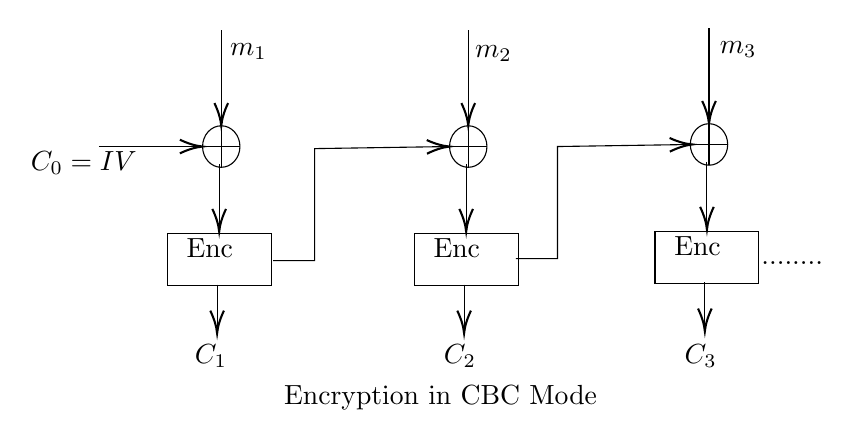
\begin{tikzpicture}[x=0.75pt,y=0.75pt,yscale=-1,xscale=1]
        \draw   (100,123) .. controls (100,117.48) and (104.03,113) .. (109,113) .. controls (113.97,113) and (118,117.48) .. (118,123) .. controls (118,128.52) and (113.97,133) .. (109,133) .. controls (104.03,133) and (100,128.52) .. (100,123) -- cycle ; \draw   (100,123) -- (118,123) ; \draw   (109,113) -- (109,133) ;
        \draw    (109,67) -- (109,111) ;
        \draw [shift={(109,113)}, rotate = 270] [color={rgb, 255:red, 0; green, 0; blue, 0 }  ][line width=0.75]    (10.93,-3.29) .. controls (6.95,-1.4) and (3.31,-0.3) .. (0,0) .. controls (3.31,0.3) and (6.95,1.4) .. (10.93,3.29)   ;
        \draw   (83,165) -- (133,165) -- (133,190) -- (83,190) -- cycle ; 
        \draw    (108,131.5) -- (108,162) ;
        \draw [shift={(108,164)}, rotate = 270] [color={rgb, 255:red, 0; green, 0; blue, 0 }  ][line width=0.75]    (10.93,-3.29) .. controls (6.95,-1.4) and (3.31,-0.3) .. (0,0) .. controls (3.31,0.3) and (6.95,1.4) .. (10.93,3.29)   ;
        \draw    (107,189.5) -- (107,211) ;
        \draw [shift={(107,213)}, rotate = 270] [color={rgb, 255:red, 0; green, 0; blue, 0 }  ][line width=0.75]    (10.93,-3.29) .. controls (6.95,-1.4) and (3.31,-0.3) .. (0,0) .. controls (3.31,0.3) and (6.95,1.4) .. (10.93,3.29)   ;
        \draw   (219,123) .. controls (219,117.48) and (223.03,113) .. (228,113) .. controls (232.97,113) and (237,117.48) .. (237,123) .. controls (237,128.52) and (232.97,133) .. (228,133) .. controls (223.03,133) and (219,128.52) .. (219,123) -- cycle ; \draw   (219,123) -- (237,123) ; \draw   (228,113) -- (228,133) ;
        \draw    (228,67) -- (228,111) ;
        \draw [shift={(228,113)}, rotate = 270] [color={rgb, 255:red, 0; green, 0; blue, 0 }  ][line width=0.75]    (10.93,-3.29) .. controls (6.95,-1.4) and (3.31,-0.3) .. (0,0) .. controls (3.31,0.3) and (6.95,1.4) .. (10.93,3.29)   ;
        \draw   (202,165) -- (252,165) -- (252,190) -- (202,190) -- cycle ;
        \draw    (227,131.5) -- (227,162) ;
        \draw [shift={(227,164)}, rotate = 270] [color={rgb, 255:red, 0; green, 0; blue, 0 }  ][line width=0.75]    (10.93,-3.29) .. controls (6.95,-1.4) and (3.31,-0.3) .. (0,0) .. controls (3.31,0.3) and (6.95,1.4) .. (10.93,3.29)   ; 
        \draw    (226,189.5) -- (226,211) ;
        \draw [shift={(226,213)}, rotate = 270] [color={rgb, 255:red, 0; green, 0; blue, 0 }  ][line width=0.75]    (10.93,-3.29) .. controls (6.95,-1.4) and (3.31,-0.3) .. (0,0) .. controls (3.31,0.3) and (6.95,1.4) .. (10.93,3.29)   ;
        \draw   (335,122) .. controls (335,116.48) and (339.03,112) .. (344,112) .. controls (348.97,112) and (353,116.48) .. (353,122) .. controls (353,127.52) and (348.97,132) .. (344,132) .. controls (339.03,132) and (335,127.52) .. (335,122) -- cycle ; \draw   (335,122) -- (353,122) ; \draw   (344,112) -- (344,132) ;
        \draw    (344,66) -- (344,110) ;
        \draw [shift={(344,112)}, rotate = 270] [color={rgb, 255:red, 0; green, 0; blue, 0 }  ][line width=0.75]    (10.93,-3.29) .. controls (6.95,-1.4) and (3.31,-0.3) .. (0,0) .. controls (3.31,0.3) and (6.95,1.4) .. (10.93,3.29)   ;
        \draw   (318,164) -- (368,164) -- (368,189) -- (318,189) -- cycle ;
        \draw    (343,130.5) -- (343,161) ;
        \draw [shift={(343,163)}, rotate = 270] [color={rgb, 255:red, 0; green, 0; blue, 0 }  ][line width=0.75]    (10.93,-3.29) .. controls (6.95,-1.4) and (3.31,-0.3) .. (0,0) .. controls (3.31,0.3) and (6.95,1.4) .. (10.93,3.29)   ;
        \draw    (342,188.5) -- (342,210) ;
        \draw [shift={(342,212)}, rotate = 270] [color={rgb, 255:red, 0; green, 0; blue, 0 }  ][line width=0.75]    (10.93,-3.29) .. controls (6.95,-1.4) and (3.31,-0.3) .. (0,0) .. controls (3.31,0.3) and (6.95,1.4) .. (10.93,3.29)   ;
        \draw    (134,178) -- (154,178) -- (154,124) -- (217,123.03) ;
        \draw [shift={(219,123)}, rotate = 179.12] [color={rgb, 255:red, 0; green, 0; blue, 0 }  ][line width=0.75]    (10.93,-3.29) .. controls (6.95,-1.4) and (3.31,-0.3) .. (0,0) .. controls (3.31,0.3) and (6.95,1.4) .. (10.93,3.29)   ;
        \draw    (251,177) -- (271,177) -- (271,123) -- (334,122.03) ;
        \draw [shift={(336,122)}, rotate = 179.12] [color={rgb, 255:red, 0; green, 0; blue, 0 }  ][line width=0.75]    (10.93,-3.29) .. controls (6.95,-1.4) and (3.31,-0.3) .. (0,0) .. controls (3.31,0.3) and (6.95,1.4) .. (10.93,3.29)   ; 
        \draw    (50,123) -- (98,123) ;
        \draw [shift={(100,123)}, rotate = 180] [color={rgb, 255:red, 0; green, 0; blue, 0 }  ][line width=0.75]    (10.93,-3.29) .. controls (6.95,-1.4) and (3.31,-0.3) .. (0,0) .. controls (3.31,0.3) and (6.95,1.4) .. (10.93,3.29)   ;
        
        \draw (91,166) node [anchor=north west][inner sep=0.75pt]   [align=left] {Enc};
        \draw (95,217) node [anchor=north west][inner sep=0.75pt]   [align=left] {$C_1$};
        \draw (210,166) node [anchor=north west][inner sep=0.75pt]   [align=left] {Enc};
        \draw (215,217) node [anchor=north west][inner sep=0.75pt]   [align=left] {$C_2$};
        \draw (326,165) node [anchor=north west][inner sep=0.75pt]   [align=left] {Enc};
        \draw (331,217) node [anchor=north west][inner sep=0.75pt]   [align=left] {$C_3$};
        \draw (368,177) node [anchor=north west][inner sep=0.75pt]   [align=left] {........};
        \draw (16,124) node [anchor=north west][inner sep=0.75pt]   [align=left] {$C_0 = IV$};
        \draw (112,72) node [anchor=north west][inner sep=0.75pt]   [align=left] {$m_1$};
        \draw (230,73) node [anchor=north west][inner sep=0.75pt]   [align=left] {$m_2$};
        \draw (348,71) node [anchor=north west][inner sep=0.75pt]   [align=left] {$m_3$};
        \draw (138,237) node [anchor=north west][inner sep=0.75pt]   [align=left] {Encryption in CBC Mode};
    \end{tikzpicture}
\end{center}

\textbf{Decryption:}
\begin{center}
    $m_i = Dec(C_i, K) \oplus C_{i-1}$ $\forall$ $i \in \{1,2...,t\}$\\
    where $C_0 = IV$\\
    $M = m_1 || m_2 || ..... || m_t$
\end{center}

\begin{center}
    \tikzset{every picture/.style={line width=0.75pt}}      

    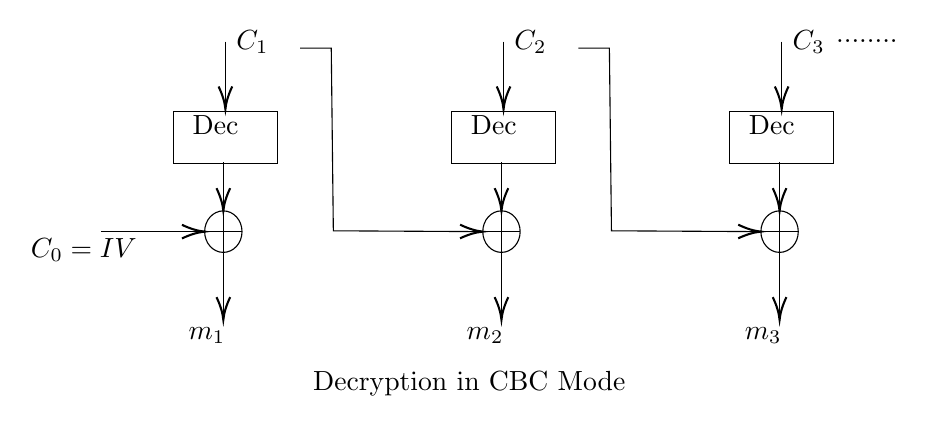
\begin{tikzpicture}[x=0.75pt,y=0.75pt,yscale=-1,xscale=1]
        \draw   (92,71) -- (142,71) -- (142,96) -- (92,96) -- cycle ; 
        \draw    (117,37.5) -- (117,68) ;
        \draw [shift={(117,70)}, rotate = 270] [color={rgb, 255:red, 0; green, 0; blue, 0 }  ][line width=0.75]    (10.93,-3.29) .. controls (6.95,-1.4) and (3.31,-0.3) .. (0,0) .. controls (3.31,0.3) and (6.95,1.4) .. (10.93,3.29)   ;
        \draw    (116,95.5) -- (116,117) ;
        \draw [shift={(116,119)}, rotate = 270] [color={rgb, 255:red, 0; green, 0; blue, 0 }  ][line width=0.75]    (10.93,-3.29) .. controls (6.95,-1.4) and (3.31,-0.3) .. (0,0) .. controls (3.31,0.3) and (6.95,1.4) .. (10.93,3.29)   ;
        \draw   (107,129) .. controls (107,123.48) and (111.03,119) .. (116,119) .. controls (120.97,119) and (125,123.48) .. (125,129) .. controls (125,134.52) and (120.97,139) .. (116,139) .. controls (111.03,139) and (107,134.52) .. (107,129) -- cycle ; \draw   (107,129) -- (125,129) ; \draw   (116,119) -- (116,139) ;
        \draw    (57,129) -- (105,129) ;
        \draw [shift={(107,129)}, rotate = 180] [color={rgb, 255:red, 0; green, 0; blue, 0 }  ][line width=0.75]    (10.93,-3.29) .. controls (6.95,-1.4) and (3.31,-0.3) .. (0,0) .. controls (3.31,0.3) and (6.95,1.4) .. (10.93,3.29)   ;
        \draw    (116,139) -- (116,169.5) ;
        \draw [shift={(116,171.5)}, rotate = 270] [color={rgb, 255:red, 0; green, 0; blue, 0 }  ][line width=0.75]    (10.93,-3.29) .. controls (6.95,-1.4) and (3.31,-0.3) .. (0,0) .. controls (3.31,0.3) and (6.95,1.4) .. (10.93,3.29)   ;
        \draw   (226,71) -- (276,71) -- (276,96) -- (226,96) -- cycle ;
        \draw    (251,37.5) -- (251,68) ;
        \draw [shift={(251,70)}, rotate = 270] [color={rgb, 255:red, 0; green, 0; blue, 0 }  ][line width=0.75]    (10.93,-3.29) .. controls (6.95,-1.4) and (3.31,-0.3) .. (0,0) .. controls (3.31,0.3) and (6.95,1.4) .. (10.93,3.29)   ;
        \draw    (250,95.5) -- (250,117) ;
        \draw [shift={(250,119)}, rotate = 270] [color={rgb, 255:red, 0; green, 0; blue, 0 }  ][line width=0.75]    (10.93,-3.29) .. controls (6.95,-1.4) and (3.31,-0.3) .. (0,0) .. controls (3.31,0.3) and (6.95,1.4) .. (10.93,3.29)   ;
        \draw   (241,129) .. controls (241,123.48) and (245.03,119) .. (250,119) .. controls (254.97,119) and (259,123.48) .. (259,129) .. controls (259,134.52) and (254.97,139) .. (250,139) .. controls (245.03,139) and (241,134.52) .. (241,129) -- cycle ; \draw   (241,129) -- (259,129) ; \draw   (250,119) -- (250,139) ;
        \draw    (250,139) -- (250,169.5) ;
        \draw [shift={(250,171.5)}, rotate = 270] [color={rgb, 255:red, 0; green, 0; blue, 0 }  ][line width=0.75]    (10.93,-3.29) .. controls (6.95,-1.4) and (3.31,-0.3) .. (0,0) .. controls (3.31,0.3) and (6.95,1.4) .. (10.93,3.29)   ;
        \draw   (360,71) -- (410,71) -- (410,96) -- (360,96) -- cycle ;
        \draw    (385,37.5) -- (385,68) ;
        \draw [shift={(385,70)}, rotate = 270] [color={rgb, 255:red, 0; green, 0; blue, 0 }  ][line width=0.75]    (10.93,-3.29) .. controls (6.95,-1.4) and (3.31,-0.3) .. (0,0) .. controls (3.31,0.3) and (6.95,1.4) .. (10.93,3.29)   ;
        \draw    (384,95.5) -- (384,117) ;
        \draw [shift={(384,119)}, rotate = 270] [color={rgb, 255:red, 0; green, 0; blue, 0 }  ][line width=0.75]    (10.93,-3.29) .. controls (6.95,-1.4) and (3.31,-0.3) .. (0,0) .. controls (3.31,0.3) and (6.95,1.4) .. (10.93,3.29)   ;
        \draw   (375,129) .. controls (375,123.48) and (379.03,119) .. (384,119) .. controls (388.97,119) and (393,123.48) .. (393,129) .. controls (393,134.52) and (388.97,139) .. (384,139) .. controls (379.03,139) and (375,134.52) .. (375,129) -- cycle ; \draw   (375,129) -- (393,129) ; \draw   (384,119) -- (384,139) ;
        \draw    (384,139) -- (384,169.5) ;
        \draw [shift={(384,171.5)}, rotate = 270] [color={rgb, 255:red, 0; green, 0; blue, 0 }  ][line width=0.75]    (10.93,-3.29) .. controls (6.95,-1.4) and (3.31,-0.3) .. (0,0) .. controls (3.31,0.3) and (6.95,1.4) .. (10.93,3.29)   ;
        \draw    (153,40.6) -- (168,40.6) -- (169,128.6) -- (239,128.99) ;
        \draw [shift={(241,129)}, rotate = 180.32] [color={rgb, 255:red, 0; green, 0; blue, 0 }  ][line width=0.75]    (10.93,-3.29) .. controls (6.95,-1.4) and (3.31,-0.3) .. (0,0) .. controls (3.31,0.3) and (6.95,1.4) .. (10.93,3.29)   ;
        \draw    (287,40.6) -- (302,40.6) -- (303,128.6) -- (373,128.99) ;
        \draw [shift={(375,129)}, rotate = 180.32] [color={rgb, 255:red, 0; green, 0; blue, 0 }  ][line width=0.75]    (10.93,-3.29) .. controls (6.95,-1.4) and (3.31,-0.3) .. (0,0) .. controls (3.31,0.3) and (6.95,1.4) .. (10.93,3.29)   ;
        
        \draw (100,72) node [anchor=north west][inner sep=0.75pt]   [align=left] {Dec};
        \draw (121,31) node [anchor=north west][inner sep=0.75pt]   [align=left] {$C_1$};
        \draw (22,131) node [anchor=north west][inner sep=0.75pt]   [align=left] {$C_0 = IV$};
        \draw (98,174) node [anchor=north west][inner sep=0.75pt]   [align=left] {$m_1$};
        \draw (234,72) node [anchor=north west][inner sep=0.75pt]   [align=left] {Dec};
        \draw (255,31) node [anchor=north west][inner sep=0.75pt]   [align=left] {$C_2$};
        \draw (232,174) node [anchor=north west][inner sep=0.75pt]   [align=left] {$m_2$};
        \draw (368,72) node [anchor=north west][inner sep=0.75pt]   [align=left] {Dec};
        \draw (389,31) node [anchor=north west][inner sep=0.75pt]   [align=left] {$C_3$};
        \draw (366,174) node [anchor=north west][inner sep=0.75pt]   [align=left] {$m_3$};
        \draw (410,35) node [anchor=north west][inner sep=0.75pt]   [align=left] {........};
        \draw (158,195) node [anchor=north west][inner sep=0.75pt]   [align=left] {Decryption in CBC Mode};

    \end{tikzpicture}
\end{center}

\subsection*{Stream Cipher}
Stream ciphers encrypt bitwise. 

Let \( M = m_0 m_1 \ldots m_i \) where \( m_i \in \{0, 1\} \) represents the plaintext. 

Let \( K = k_0 k_1 \ldots k_i \) represent the key. 

The ciphertext \( C \) is obtained by bitwise XOR (exclusive or) operation: 

\[ C = M \oplus K = c_0 c_1 \ldots c_i \] 
where \( c_i = m_i \oplus k_i \).


\subsection*{Shannon’s Notion of Perfect Secrecy}

Perfect secrecy, as defined by Claude Shannon, ensures that the ciphertext provides no information about the plaintext. This is expressed as:
\[ P[M = M_1 | C = CH_1] = P[M = M_1] \]
If this condition holds, the algorithm is considered perfectly secure, meaning the ciphertext reveals nothing about the plaintext.

\subsection*{Conditions for Perfect Secrecy in Stream Cipher}

To achieve perfect secrecy in a stream cipher, the following conditions must be satisfied:
\begin{enumerate}
    \item \textbf{Key Length:} The length of the key must be greater than or equal to the length of the message.
    \item \textbf{Unique Keys:} The same key should not be used to encrypt different messages. Each message requires a unique key, adhering to the concept of One Time Padding.
\end{enumerate}

Perfect secrecy, when implemented in a stream cipher with these conditions, ensures a high level of security by preventing the ciphertext from revealing any information about the plaintext.



\end{document}
